\section{Supplementary Material}
\label{sec:Supplementary}
 \begin{figure}[htb]
    \renewcommand{\thesubfigure}{\arabic{row}.\alph{subfigure}}%
 	\centering
    \setcounter{row}{1}%
 	\subfloat[]{
 		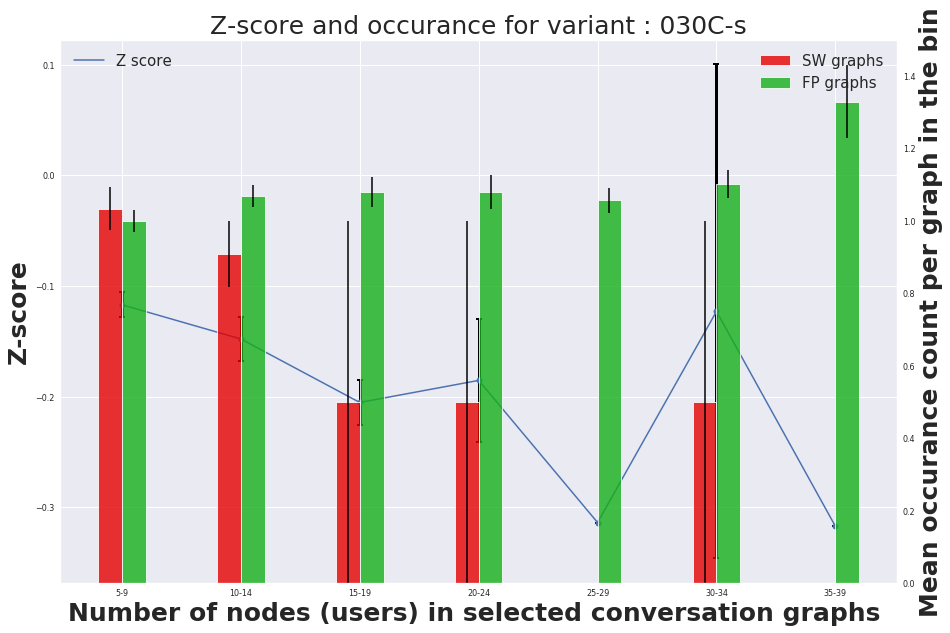
\includegraphics[width=0.25\textwidth]{Figures/Zscore/030C-a.png}
 	}
 	\subfloat[]{
 		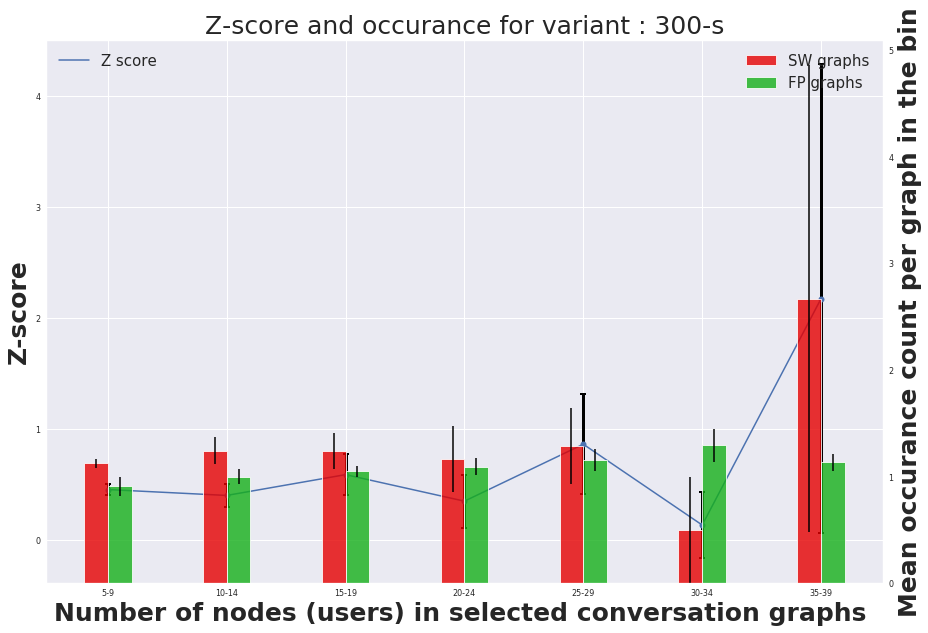
\includegraphics[width=0.25\textwidth ]{Figures/Zscore/300-s.png}
 	}
 	\subfloat[]{
 		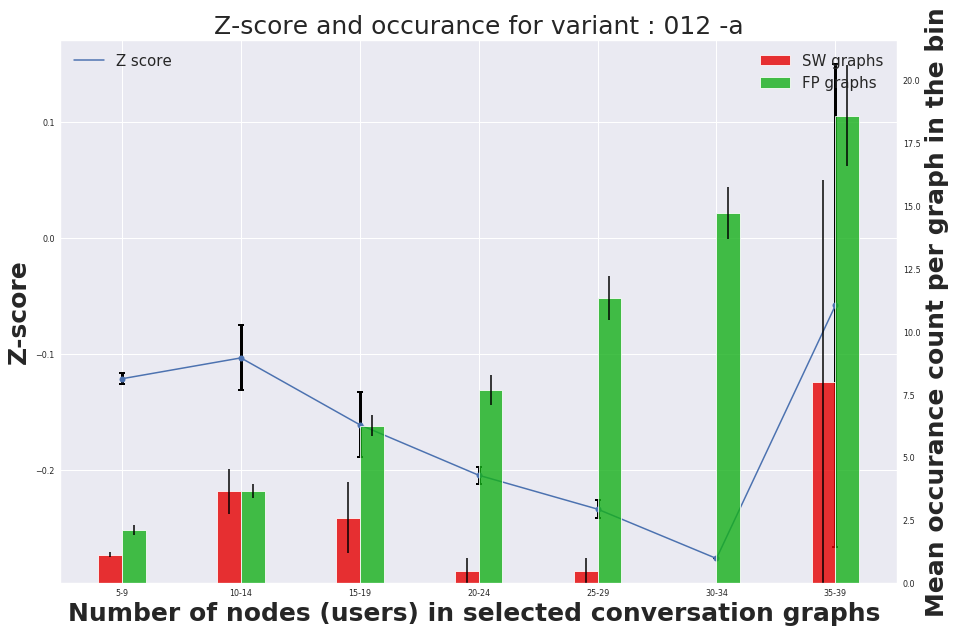
\includegraphics[width=0.25\textwidth]{Figures/Zscore/012-a.png}
 	}


    \stepcounter{row}%
 	\subfloat[]{
 	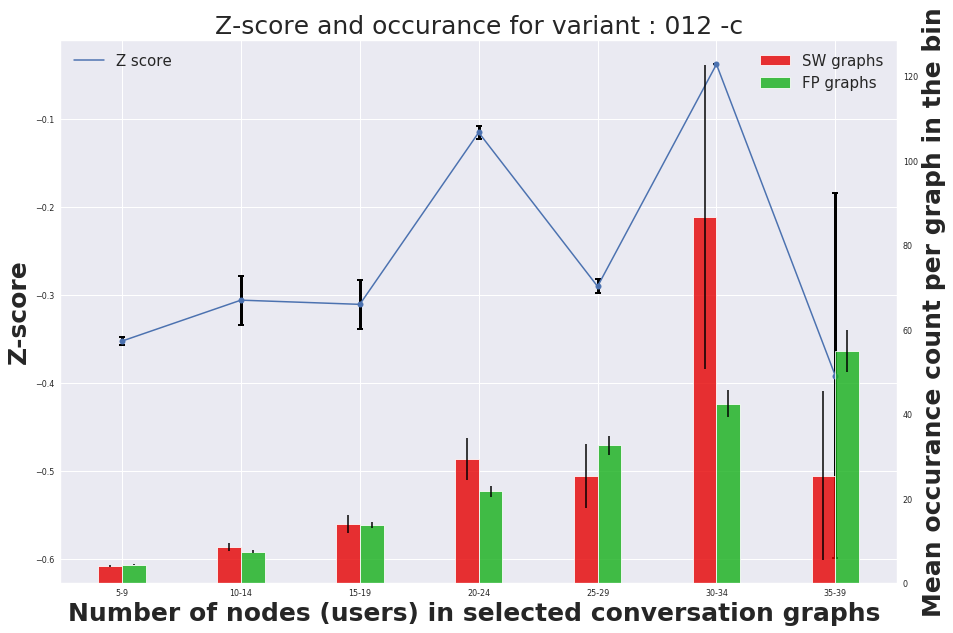
\includegraphics[width=0.25\textwidth ]{Figures/Zscore/012-c.png}
 	}
 	\subfloat[]{
 	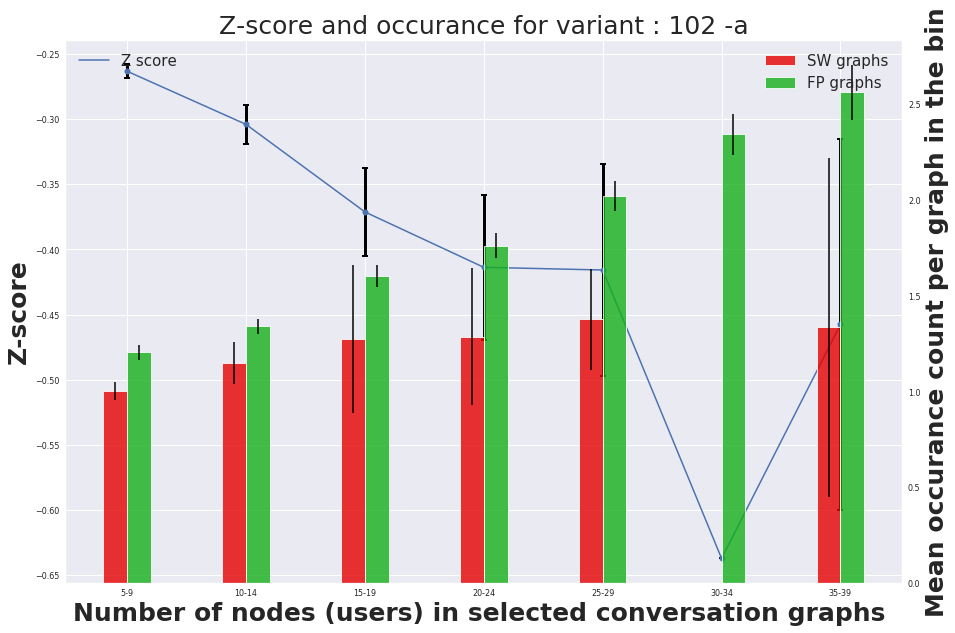
\includegraphics[width=0.25\textwidth]{Figures/Zscore/102-a.png}
 	}
    \subfloat[]{
 	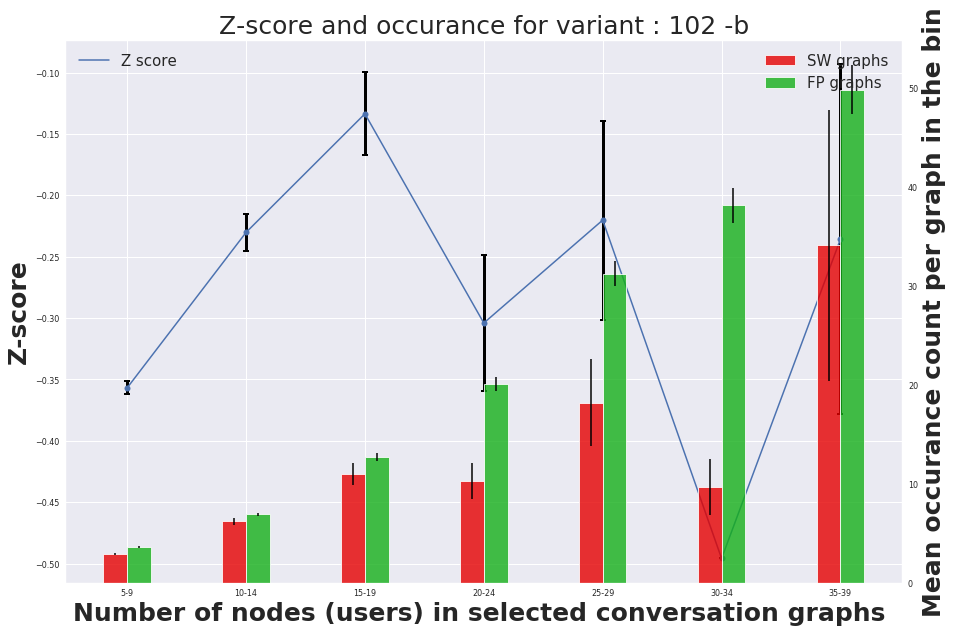
\includegraphics[width=0.25\textwidth]{Figures/Zscore/102-b.png}
 	}
	
    \stepcounter{row}%
    \subfloat[]{
 	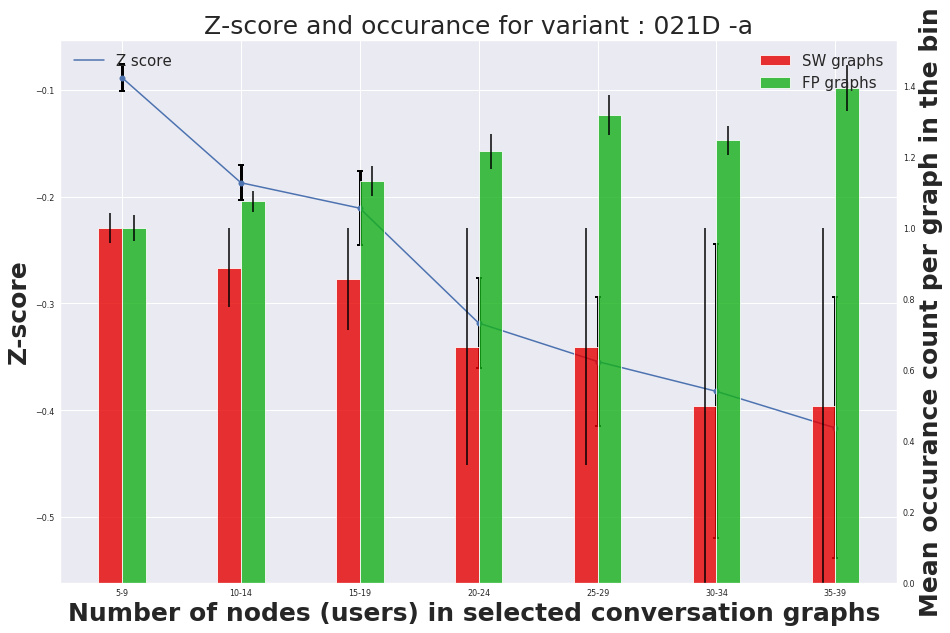
\includegraphics[width=0.25\textwidth ]{Figures/Zscore/021D-a.png}
 	}
 	\subfloat[]{
 	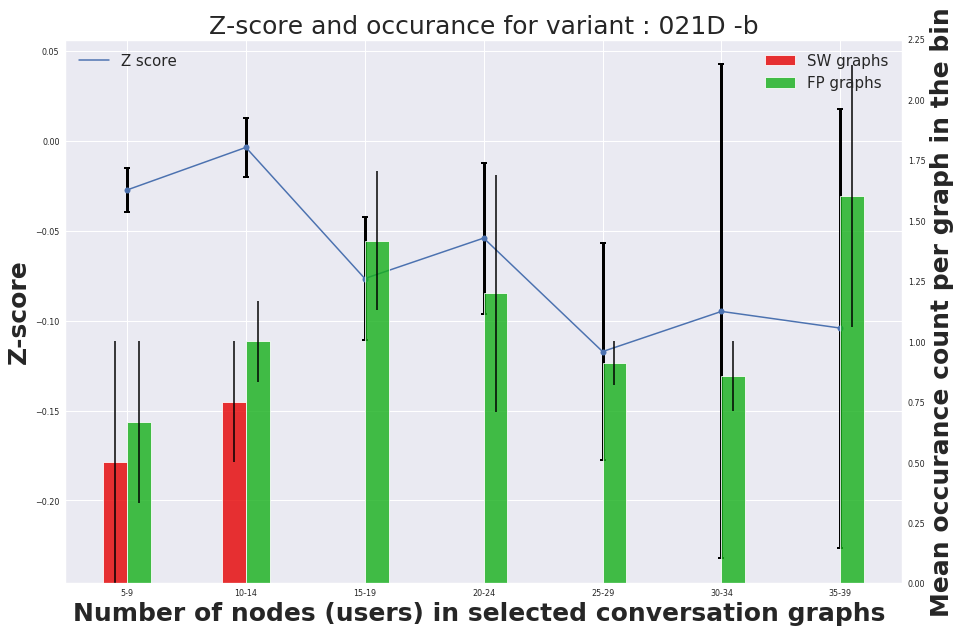
\includegraphics[width=0.25\textwidth ]{Figures/Zscore/021D-b.png}
 	}
    \subfloat[]{
 	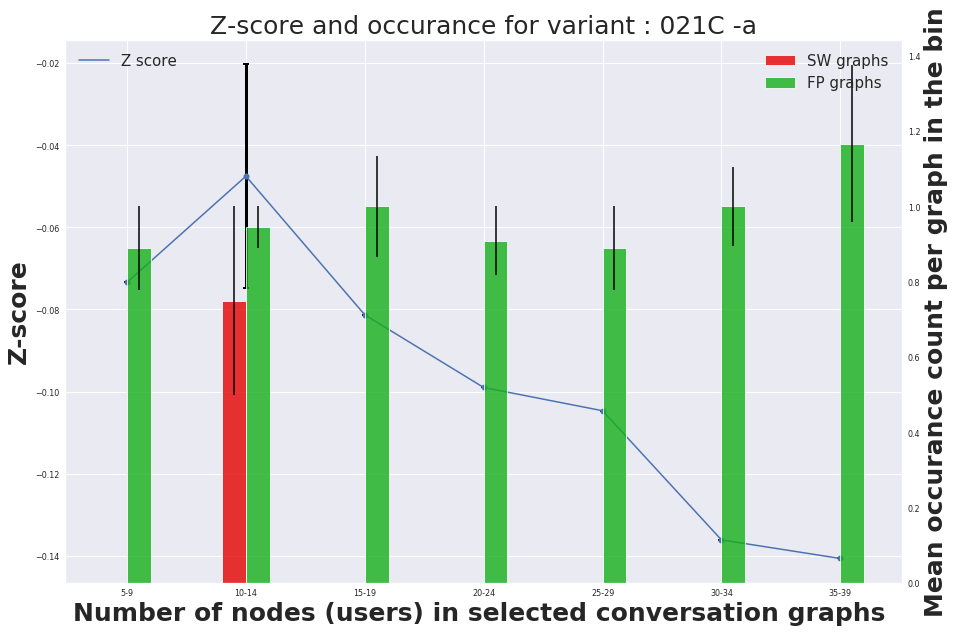
\includegraphics[width=0.25\textwidth]{Figures/Zscore/021C-a.png}
 	}
	
    
    \stepcounter{row}%
 	\subfloat[]{
 	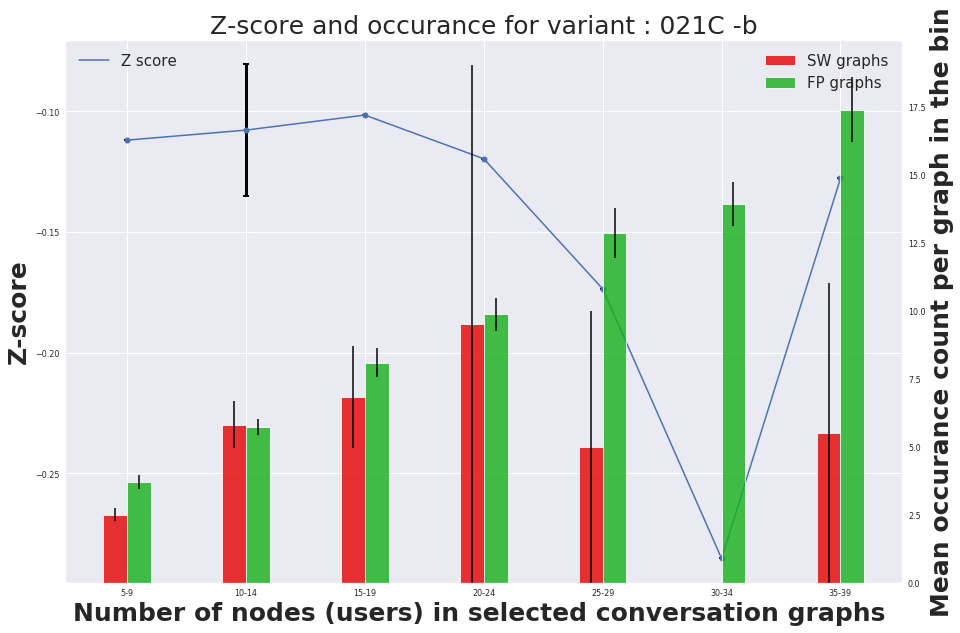
\includegraphics[width=0.25\textwidth]{Figures/Zscore/021C-b.png}
 	}
 	\subfloat[]{
 	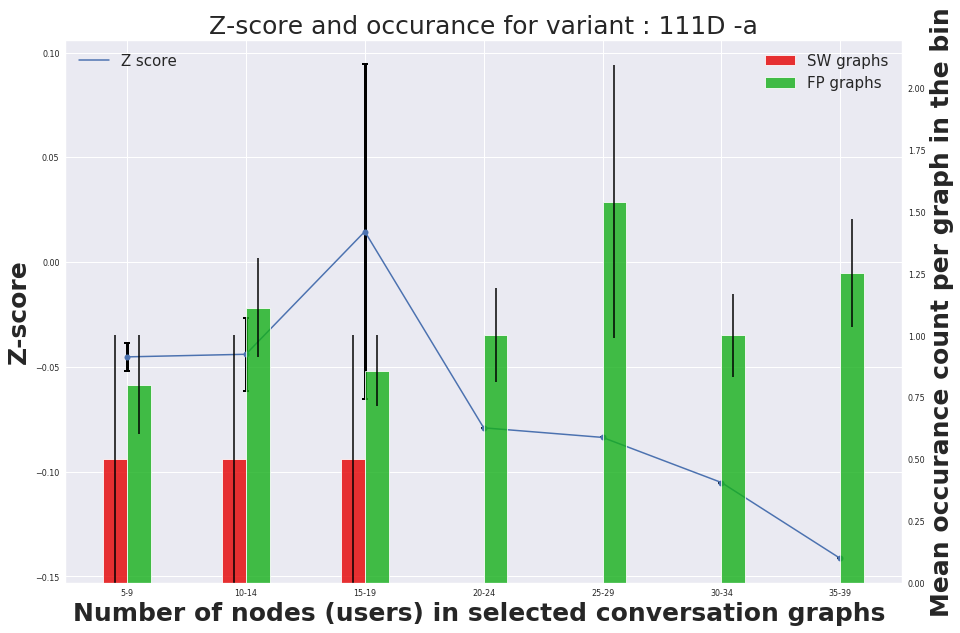
\includegraphics[width=0.25\textwidth ]{Figures/Zscore/111D-a.png}
 	}
 	\subfloat[]{
 	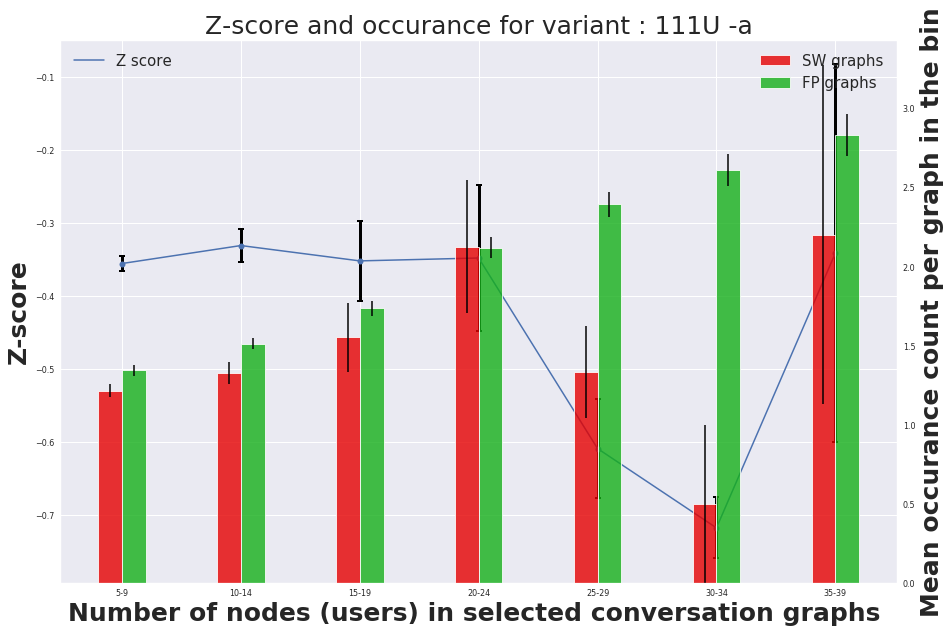
\includegraphics[width=0.25\textwidth ]{Figures/Zscore/111U-a.png}
 	}
    
    
    \stepcounter{row}%
   	\subfloat[]{
    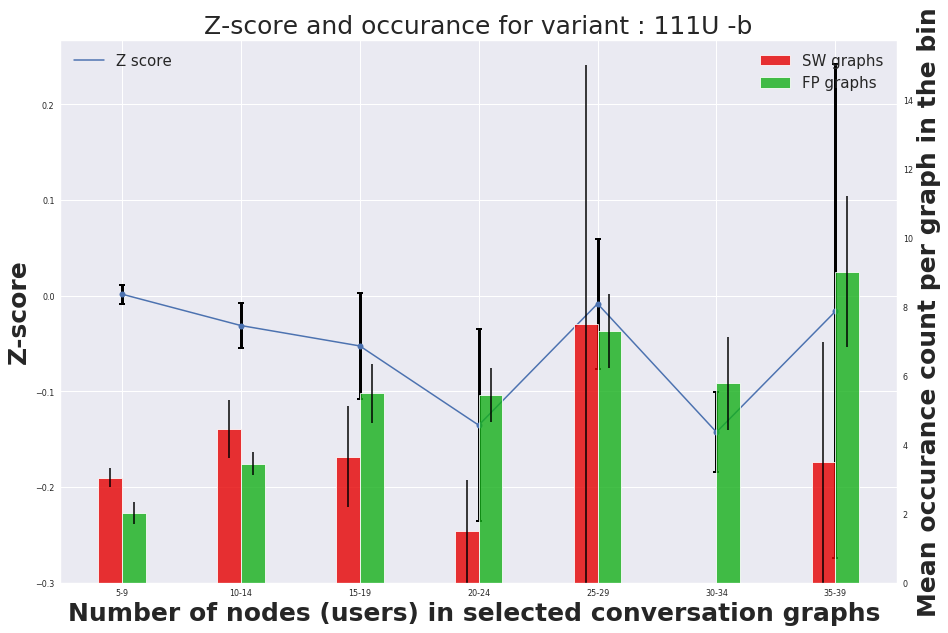
\includegraphics[width=0.25\textwidth]{Figures/Zscore/111U-b.png}
    }
    \subfloat[]{
    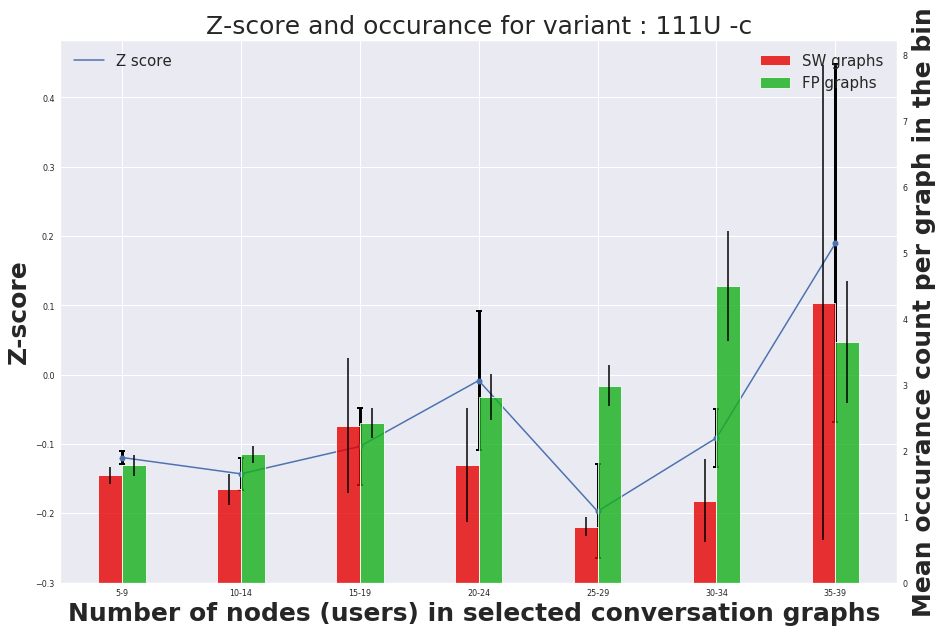
\includegraphics[width=0.25\textwidth ]{Figures/Zscore/111U-c.png}
    }
    \subfloat[]{
    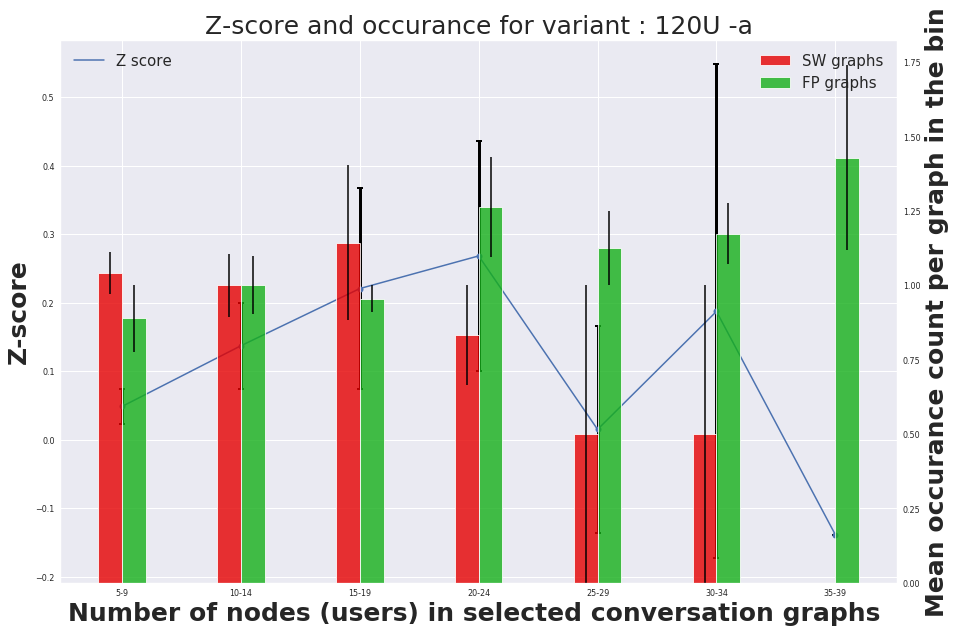
\includegraphics[width=0.25\textwidth]{Figures/Zscore/120U-a.png}
    }
 \end{figure}


 \begin{figure}[htb]\ContinuedFloat
    \renewcommand{\thesubfigure}{\arabic{row}.\alph{subfigure}}%
 	\centering
     
    \setcounter{row}{6}%
 	\subfloat[]{
 	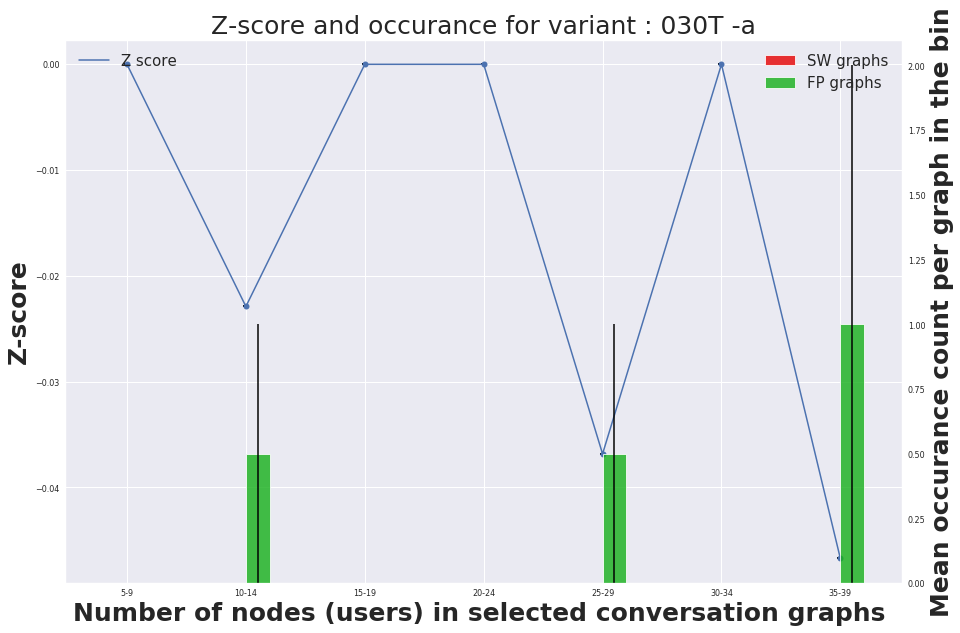
\includegraphics[width=0.25\textwidth]{Figures/Zscore/030T-a.png}
 	}
 	\subfloat[]{
 	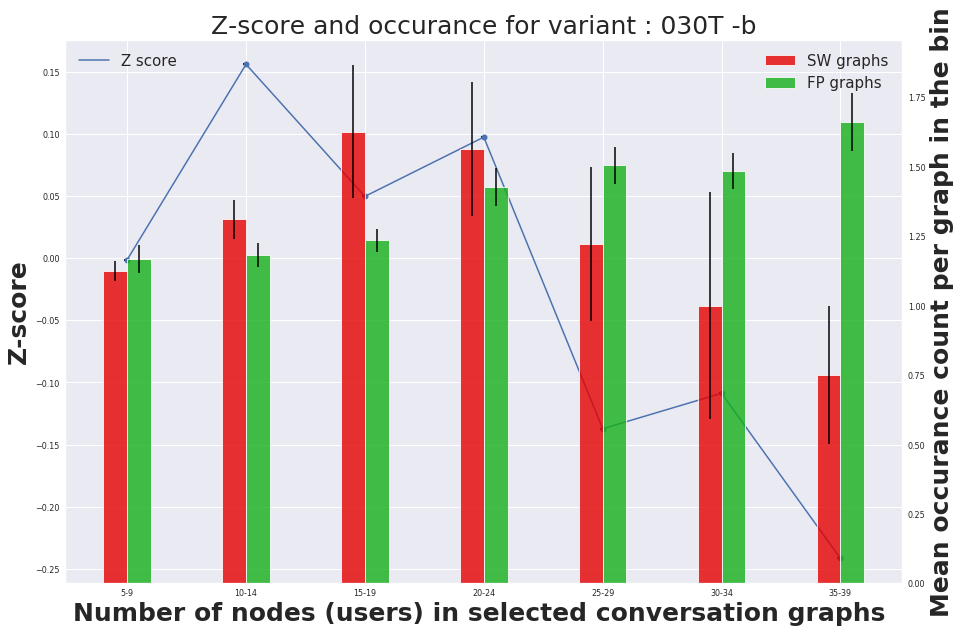
\includegraphics[width=0.25\textwidth ]{Figures/Zscore/030T-b.png}
 	}
 	\subfloat[]{
 	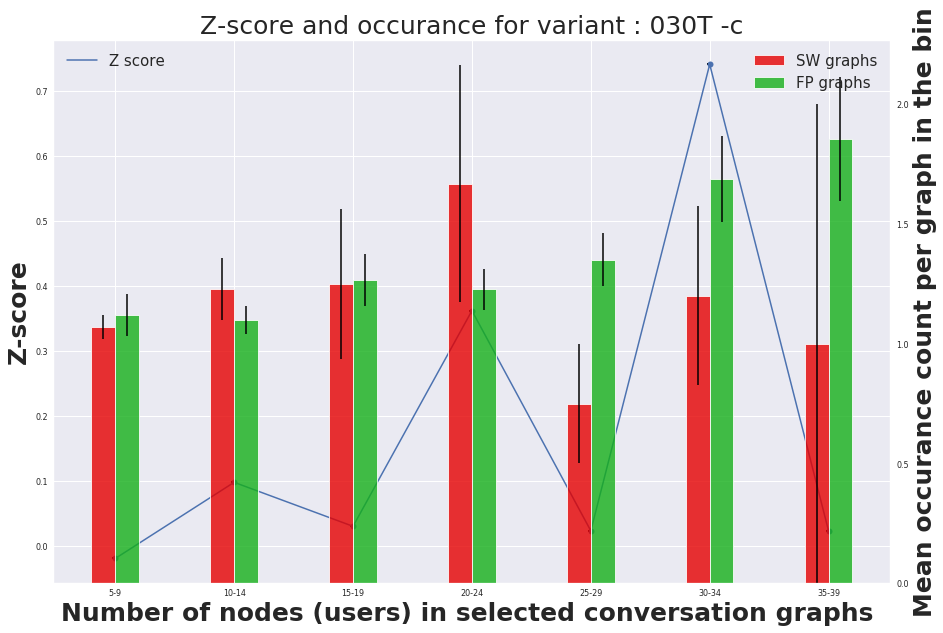
\includegraphics[width=0.25\textwidth]{Figures/Zscore/030T-c.png}
 	}
	
    \stepcounter{row}%
 	\subfloat[]{
 	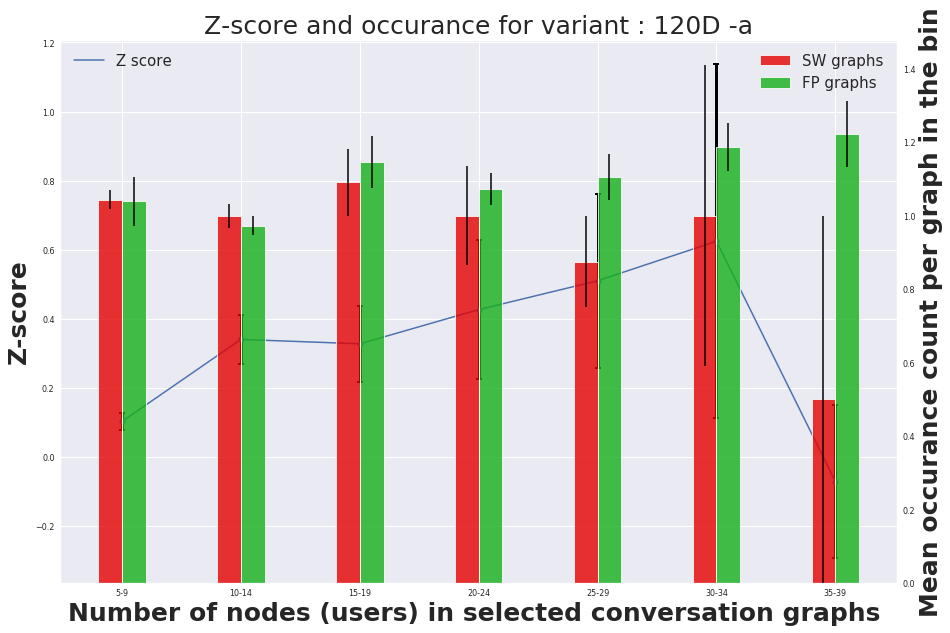
\includegraphics[width=0.25\textwidth]{Figures/Zscore/120D-a.png}
 	}
 	\subfloat[]{
 	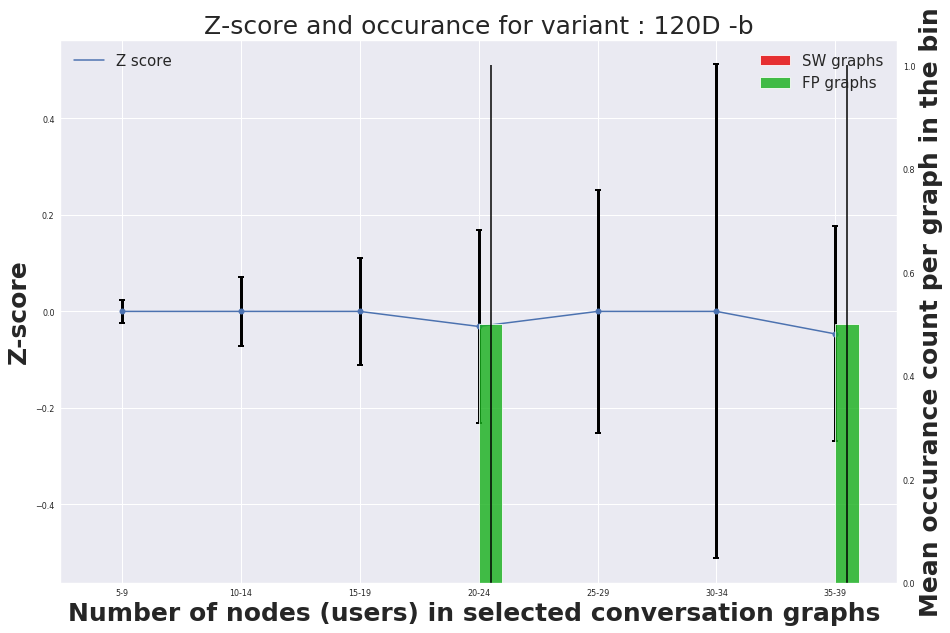
\includegraphics[width=0.25\textwidth ]{Figures/Zscore/120D-b.png}
 	}
 	\subfloat[]{
 	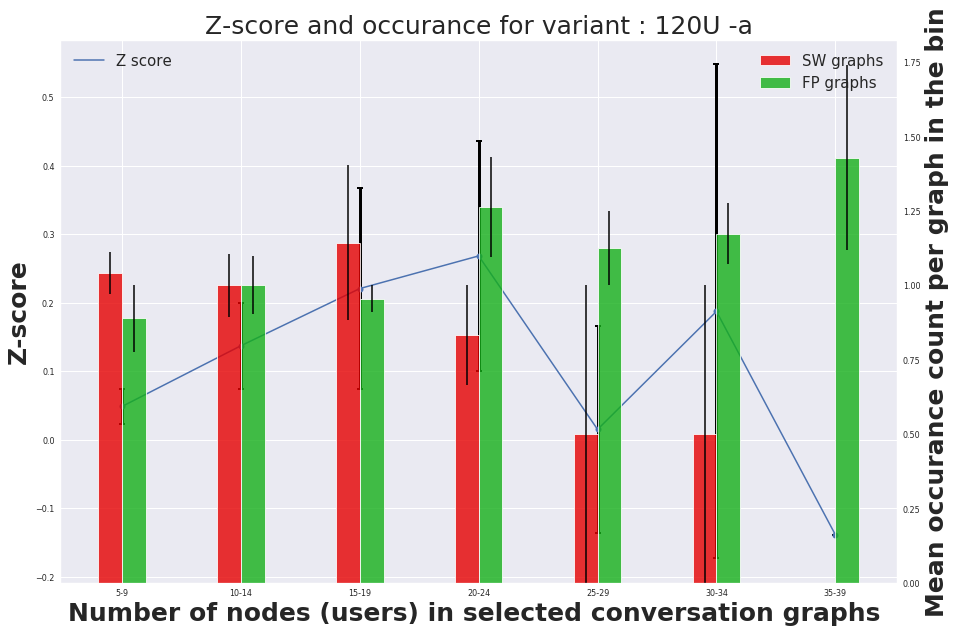
\includegraphics[width=0.25\textwidth ]{Figures/Zscore/120U-a.png}
 	}
	
    \stepcounter{row}%
    \subfloat[]{
    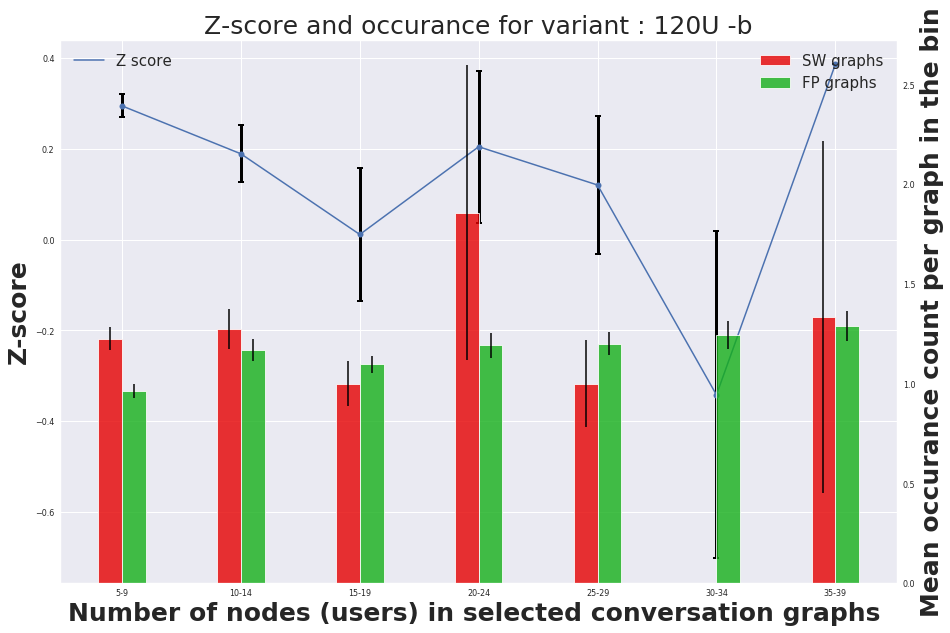
\includegraphics[width=0.25\textwidth ]{Figures/Zscore/120U-b.png}
    }
	\subfloat[]{
    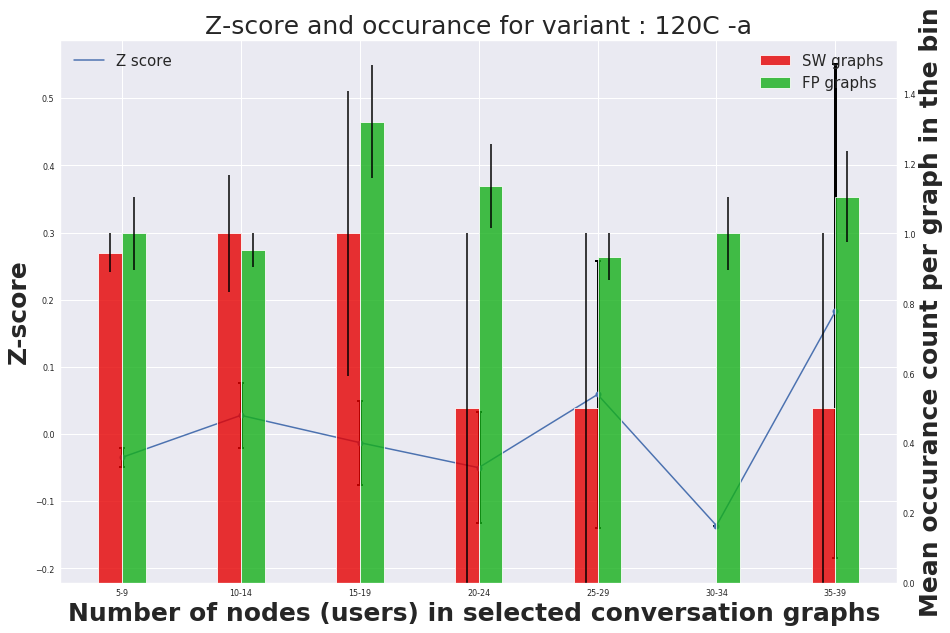
\includegraphics[width=0.25\linewidth ]{Figures/Zscore/120C-a.png}
    }
	\subfloat[]{
    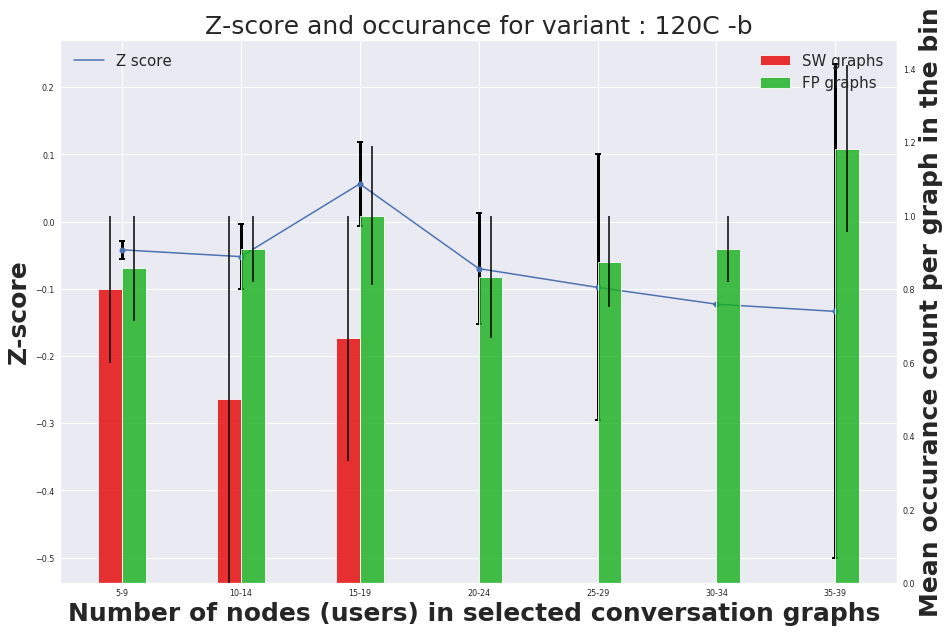
\includegraphics[width=0.25\linewidth ]{Figures/Zscore/120C-b.png}
    }


    \stepcounter{row}%
    \subfloat[]{
    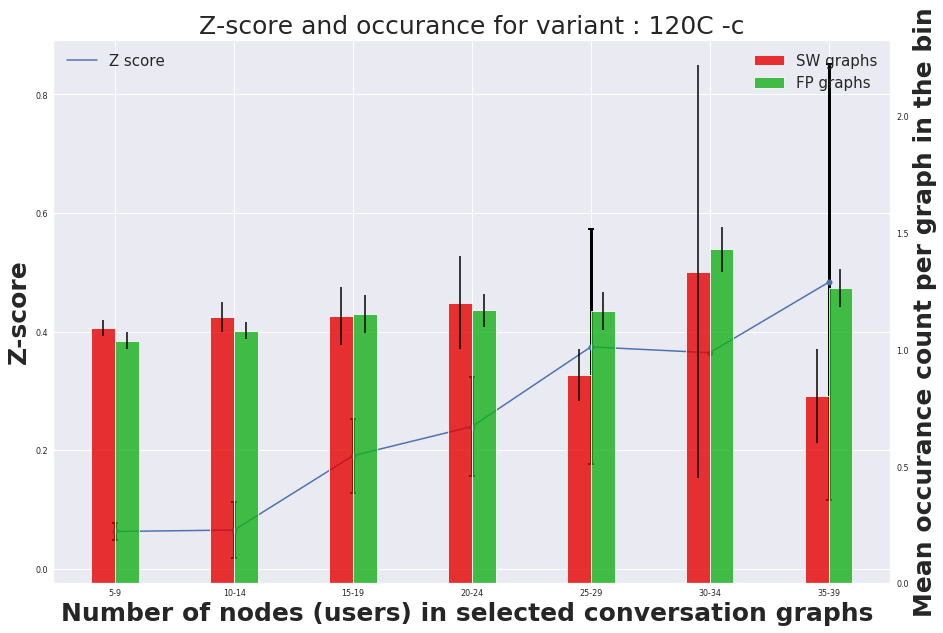
\includegraphics[width=0.25\textwidth ]{Figures/Zscore/120C-c.png}
    }
    \subfloat[]{
    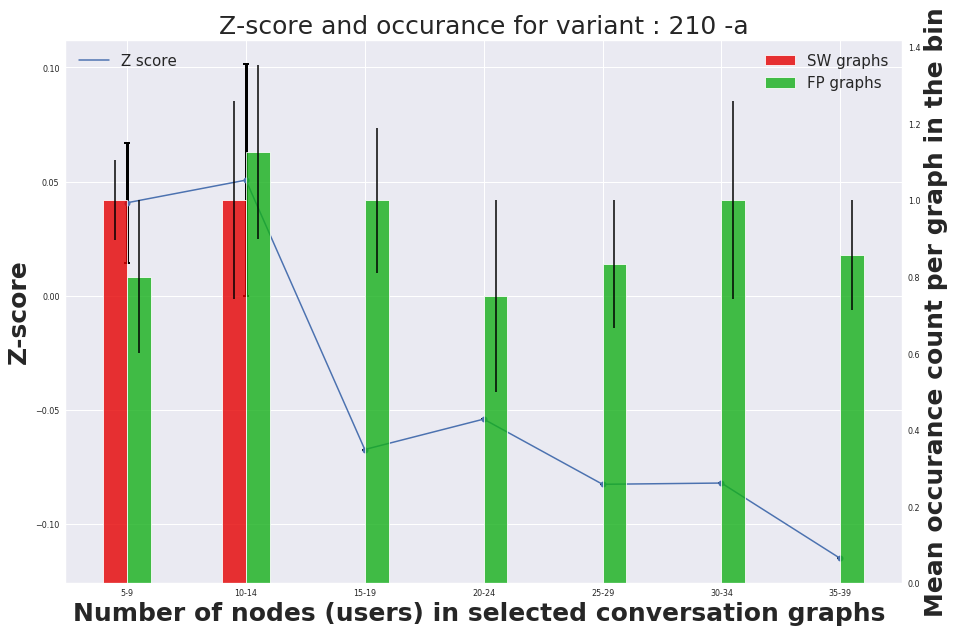
\includegraphics[width=0.25\linewidth ]{Figures/Zscore/210-a.png}
    }
    \subfloat[]{
    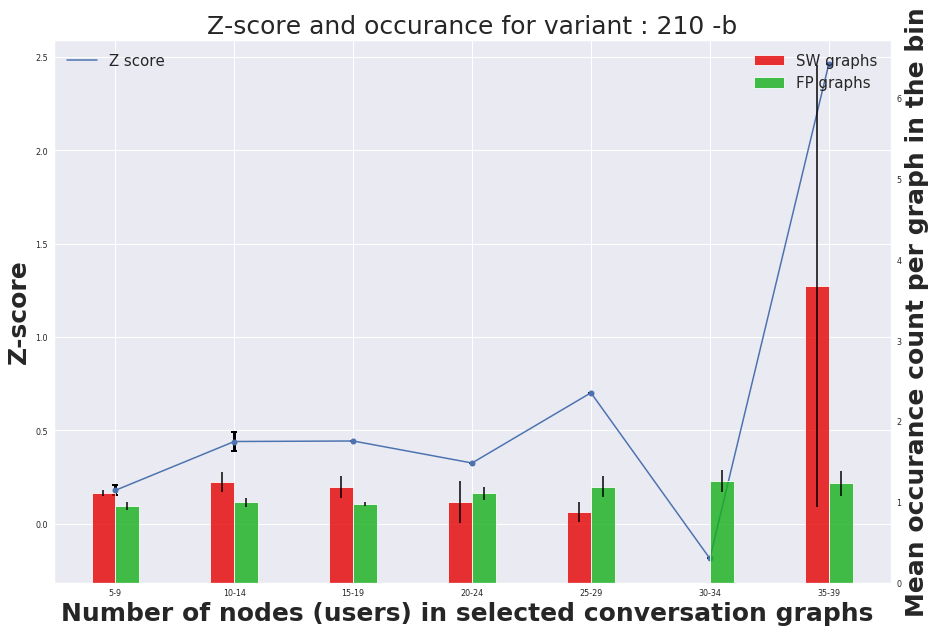
\includegraphics[width=0.25\linewidth ]{Figures/Zscore/210-b.png}
    }
    
    \stepcounter{row}%
    \subfloat[]{
    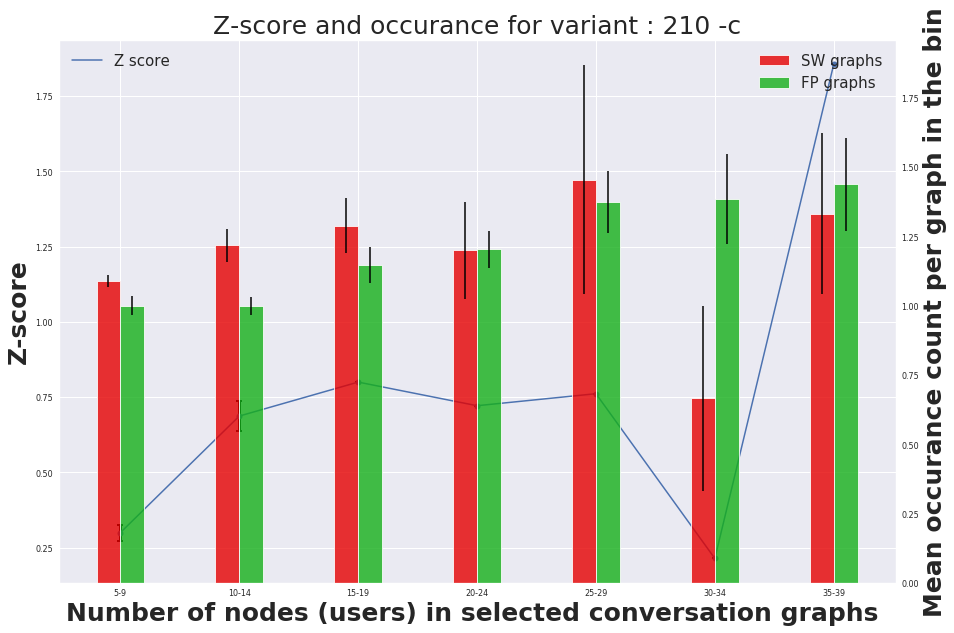
\includegraphics[width=0.25\linewidth ]{Figures/Zscore/210-c.png}
    }
 	\caption{ This figure lists all the insignificant Anchored motifs, either by the virtue of rare occurrence ($<$10 mean motifs per bin) or by account of low Z-score ($\left|Z\right|  < 1$).}
 	 \label{fig:Rare_motifs}
 \end{figure}





% \subsection{Network characteristics}
% Figure \nameref{fig:depthDist} shows the distribution of maximum depths across all Reply graphs for SW and FP subreddits. The SW threads depths have a median depth of 2 and mean of 4 compared to median depth of 2 for FP and a mean of 2.5. This shows that statistically the depths of SW and FP graphs are quite similar.


% \begin{figure}[!ht]
%     \centering
%     % \hspace*{-5mm}
%     \subfloat[]{
%         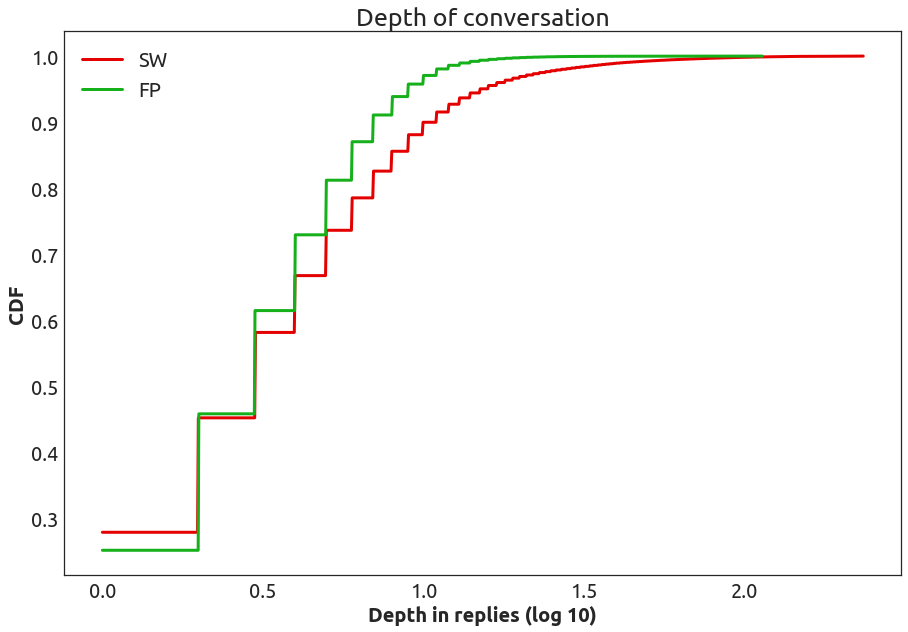
\includegraphics[width=0.4\textwidth]{Figures/V1/ConvDepth.png}
%         \label{fig:depthDist} }	
%     \subfloat[]{
%         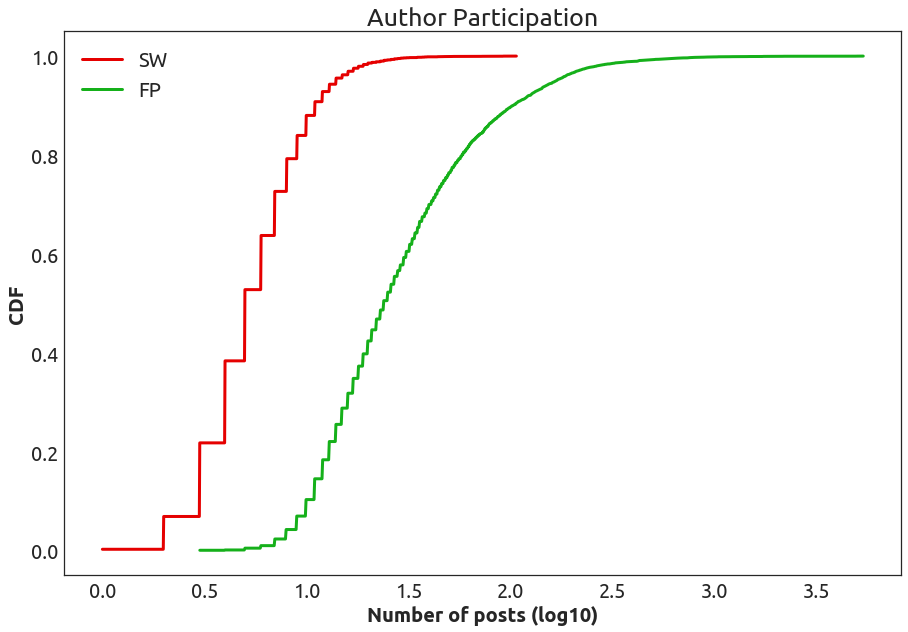
\includegraphics[width=0.4\linewidth ]{Figures/V1/AuthorParticipation.png}
%         \label{fig:uniqAuthors}
%     }
    
    
%     \subfloat[]{
%         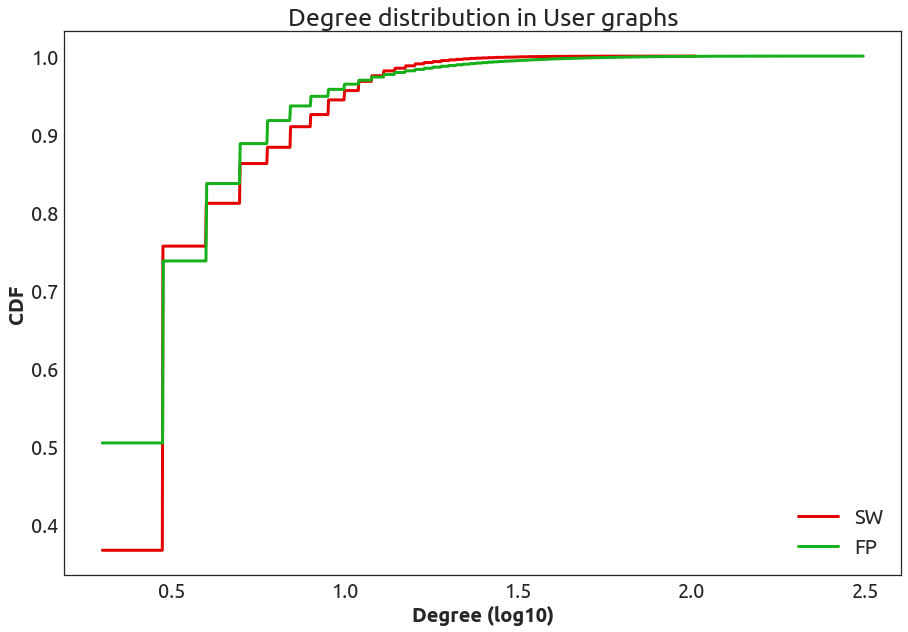
\includegraphics[width=0.4\textwidth ]{Figures/V1/UserDegDist.png}
%         \label{fig:degUgraph}
%     }
%     \subfloat[]{
%         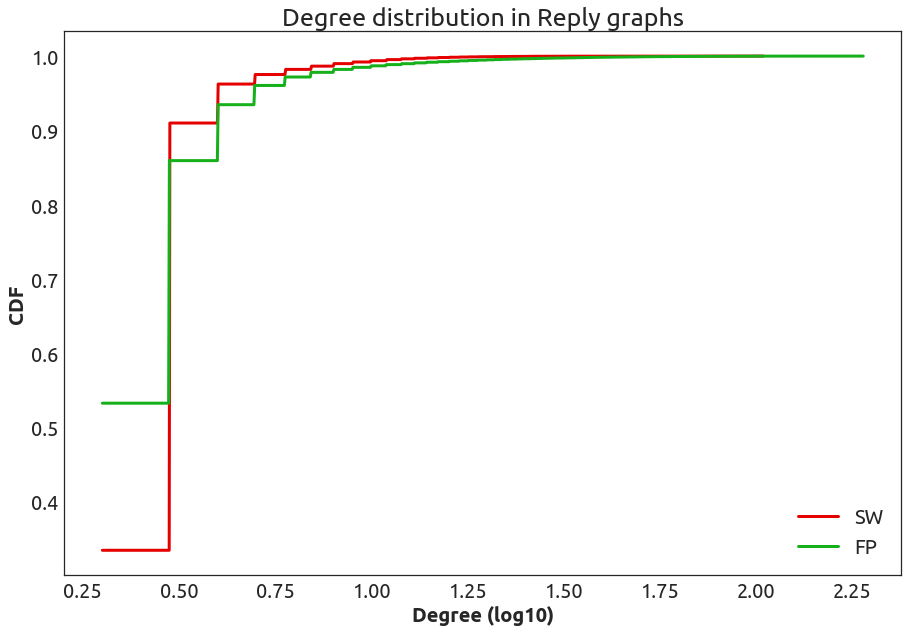
\includegraphics[width=0.4\linewidth]{Figures/V1/ReplyDegDist.png}
%         \label{fig:degRgraph}
%     }
%     \caption{\textsl{ \ref{fig:depthDist} shows the distribution of maximum depths of Reply Graphs for SW and the FP conversations. \ref{fig:uniqAuthors} shows the distribution of unique authors per thread in the two datasets. \ref{fig:degRgraph} shows Distribution of degrees for Reply Graphs, SW and FP. \ref{fig:degUgraph} shows the degree distributions for the reply graphs}}
% \end{figure}

% Figure\nameref{fig:responseDist} shows the CDF for the number of responses a Root post gets on a thread across the whole dataset. 